% Mapa Iridológico — versão moderna e limpa
% Compile: pdflatex iris_organsysteme.tex   (ou cole no Overleaf)
\documentclass[tikz,border=14pt]{standalone}
\usepackage[utf8]{inputenc}
\usepackage[T1]{fontenc}
\usepackage{lmodern}
\usepackage{tikz}
\usetikzlibrary{calc,backgrounds}

% =================== PALETA MODERNA ===================
\definecolor{cBg}      {RGB}{248,250,252}
\definecolor{cTitle}   {RGB}{15,42,86}
\definecolor{cSub}     {RGB}{100,116,139}
\definecolor{cRing}    {RGB}{226,232,240}
\definecolor{cIris1}   {RGB}{186,214,236}
\definecolor{cIris2}   {RGB}{96,150,196}
\definecolor{cIris3}   {RGB}{52,103,156}
\definecolor{cPupil}   {RGB}{38,52,74}
\definecolor{cAccent}  {RGB}{220,90,80}
\definecolor{cLabel}   {RGB}{30,41,59}
\definecolor{cLine}    {RGB}{148,163,184}

% =================== GEOMETRIA ===================
\def\hr#1{90-30*(#1)}      % hora -> ângulo
\def\Rpupil{0.85}
\def\Riris{2.55}           % raio externo da íris (azul)
\def\Rring{2.75}           % raio externo do anel claro
\def\Rtick{2.95}           % onde terminam os "ticks" dos divisores
\def\Rdot{3.10}            % onde fica o ponto que liga ao rótulo
\def\Rlabel{3.55}          % raio onde se alinham os textos

% =================== MACRO: OLHO ===================
% #1 = x   #2 = letra (D/E)
\newcommand{\drawIris}[2]{%
  \begin{scope}[shift={(#1,0)}]
    % glow externo sutil
    \fill[cRing,opacity=0.55] (0,0) circle (\Rring+0.18);
    % anel claro de fundo
    \fill[cRing] (0,0) circle (\Rring);
    % íris em três tons (gradiente discreto)
    \fill[cIris1] (0,0) circle (\Riris);
    \fill[cIris2] (0,0) circle (\Riris*0.78);
    \fill[cIris3] (0,0) circle (\Riris*0.55);
    % pupila
    \fill[cPupil] (0,0) circle (\Rpupil);
    % brilho na pupila
    \fill[white,opacity=0.55] ($(0,0)+(135:0.30)$) circle (0.10);
    % letra central
    \node[white,font=\sffamily\Large\bfseries] at (0,0) {#2};
  \end{scope}
}

% Sub-macros para os dois lados (mais simples e robusto)
% \sectorR / \sectorL : #1 = x centro do olho, #2 = hora, #3 = texto
\newcommand{\sectorR}[3]{%
  \begin{scope}[shift={(#1,0)}]
    \pgfmathsetmacro{\yend}{sin(\hr{#2})*\Rdot}
    \pgfmathsetmacro{\xdot}{cos(\hr{#2})*\Rdot}
    \draw[cLine,line width=0.6pt] ({\hr{#2}}:\Rring) -- ({\hr{#2}}:\Rtick);
    \fill[cAccent] ({\hr{#2}}:\Rdot) circle (0.055);
    \draw[cLine,line width=0.5pt] (\xdot,\yend) -- (\Rlabel,\yend);
    \node[font=\sffamily\scriptsize,text=cLabel,anchor=west]
      at (\Rlabel+0.05,\yend) {#3};
  \end{scope}
}
\newcommand{\sectorL}[3]{%
  \begin{scope}[shift={(#1,0)}]
    \pgfmathsetmacro{\yend}{sin(\hr{#2})*\Rdot}
    \pgfmathsetmacro{\xdot}{cos(\hr{#2})*\Rdot}
    \draw[cLine,line width=0.6pt] ({\hr{#2}}:\Rring) -- ({\hr{#2}}:\Rtick);
    \fill[cAccent] ({\hr{#2}}:\Rdot) circle (0.055);
    \draw[cLine,line width=0.5pt] (\xdot,\yend) -- (-\Rlabel,\yend);
    \node[font=\sffamily\scriptsize,text=cLabel,anchor=east]
      at (-\Rlabel-0.05,\yend) {#3};
  \end{scope}
}

\begin{document}
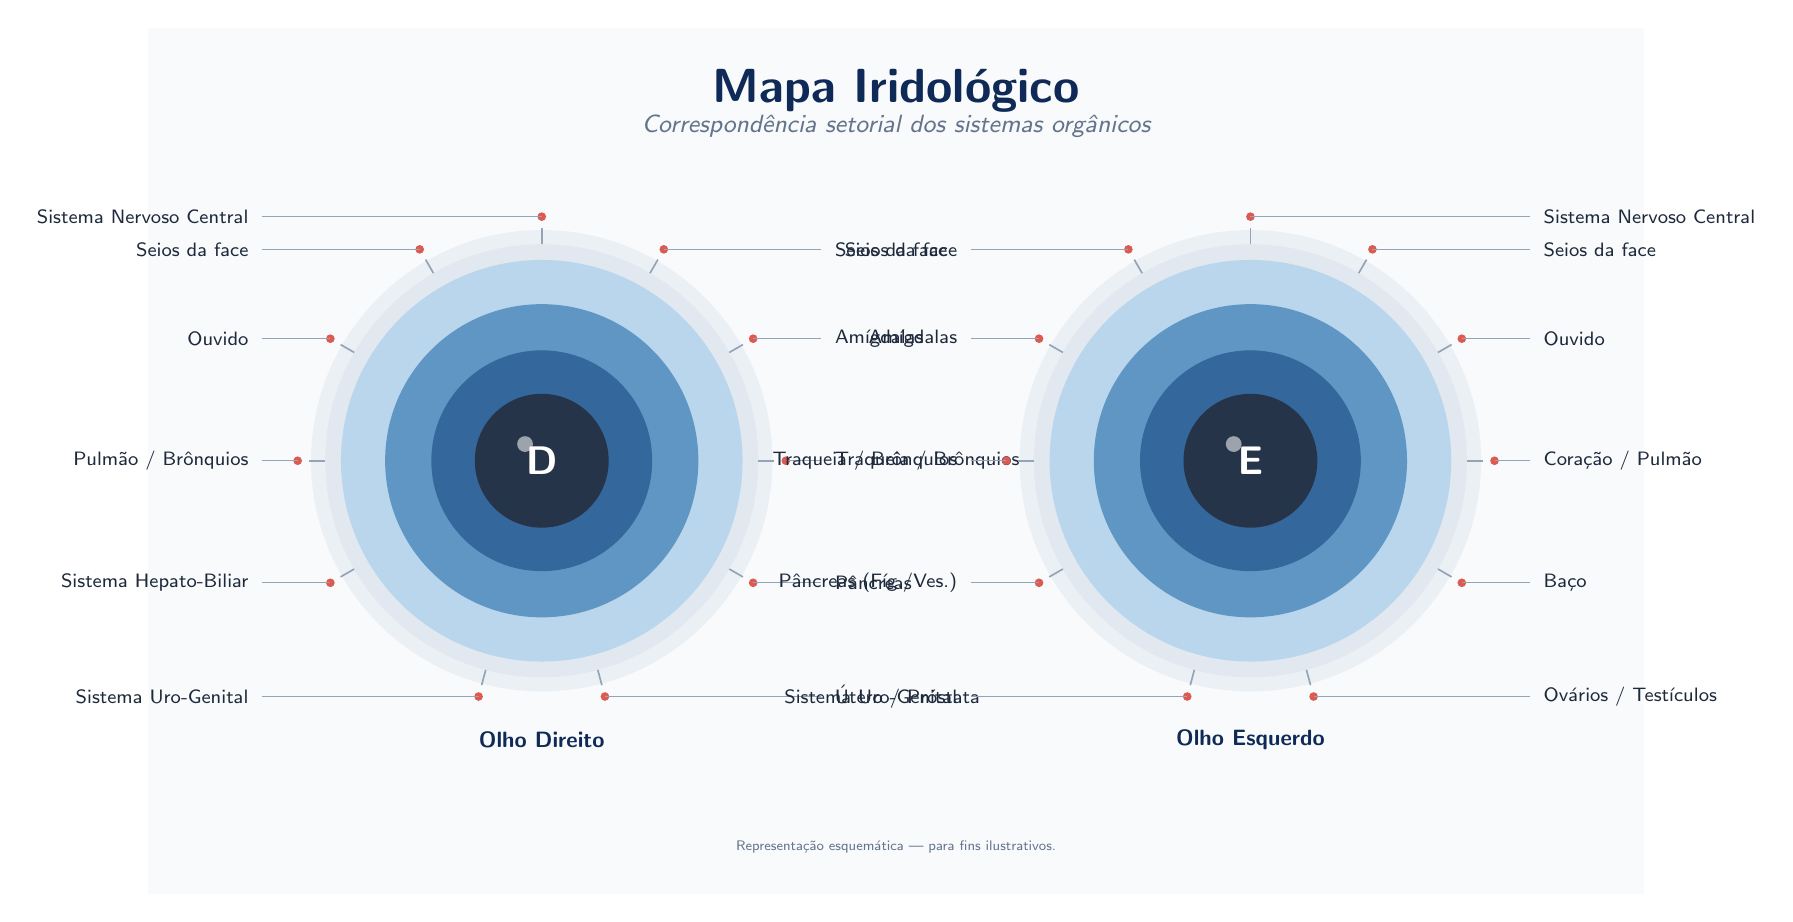
\begin{tikzpicture}[font=\sffamily]

% fundo
\begin{scope}[on background layer]
  \fill[cBg] (-9.5,-5.5) rectangle (9.5,5.5);
\end{scope}

% =================== TÍTULO ===================
\node[font=\sffamily\LARGE\bfseries,text=cTitle] at (0,4.7)
  {Mapa Iridológico};
\node[font=\sffamily\small\itshape,text=cSub] at (0,4.25)
  {Correspondência setorial dos sistemas orgânicos};

% =================== OLHO DIREITO (D) ===================
\drawIris{-4.5}{D}
% rótulos do lado esquerdo (saem para a esquerda)
\sectorL{-4.5}{12}{Sistema Nervoso Central}
\sectorL{-4.5}{11}{Seios da face}
\sectorL{-4.5}{10}{Ouvido}
\sectorL{-4.5}{9}{Pulmão / Brônquios}
\sectorL{-4.5}{8}{Sistema Hepato-Biliar}
\sectorL{-4.5}{6.5}{Sistema Uro-Genital}
% rótulos do lado direito (saem para a direita) — ficam entre os dois olhos
\sectorR{-4.5}{1}{Seios da face}
\sectorR{-4.5}{2}{Amígdalas}
\sectorR{-4.5}{3}{Traqueia / Brônquios}
\sectorR{-4.5}{4}{Pâncreas}
\sectorR{-4.5}{5.5}{Útero / Próstata}

% legenda do olho
\node[font=\sffamily\footnotesize\bfseries,text=cTitle]
  at (-4.5,-3.55) {Olho Direito};

% =================== OLHO ESQUERDO (E) ===================
\drawIris{4.5}{E}
% rótulos do lado direito (saem para a direita)
\sectorR{4.5}{12}{Sistema Nervoso Central}
\sectorR{4.5}{1}{Seios da face}
\sectorR{4.5}{2}{Ouvido}
\sectorR{4.5}{3}{Coração / Pulmão}
\sectorR{4.5}{4}{Baço}
\sectorR{4.5}{5.5}{Ovários / Testículos}
% rótulos do lado esquerdo (entre os dois olhos)
\sectorL{4.5}{11}{Seios da face}
\sectorL{4.5}{10}{Amígdalas}
\sectorL{4.5}{9}{Traqueia / Brônquios}
\sectorL{4.5}{8}{Pâncreas (Fíg./Ves.)}
\sectorL{4.5}{6.5}{Sistema Uro-Genital}

\node[font=\sffamily\footnotesize\bfseries,text=cTitle]
  at (4.5,-3.55) {Olho Esquerdo};

% =================== RODAPÉ ===================
\node[font=\sffamily\tiny,text=cSub] at (0,-4.9)
  {Representação esquemática — para fins ilustrativos.};

\end{tikzpicture}
\end{document}
